\documentclass[10pt,a4paper]{article}
\usepackage[utf8]{inputenc}
\usepackage{amsmath}
\usepackage{amsfonts}
\usepackage{amssymb}
\usepackage{graphicx}
\graphicspath{ {img/} }
\author{Gradey Cullins}
\title{Extra Credit Assignment}
\begin{document}
\maketitle

\section{}
I solved the pentadiagonal matrix using the following sizes of N: \\

\noindent
N = [10 100 1000 5000 8000 10000]; \\

\noindent
By running the function \emph{solve\_penta\_sys}, files named pent\_sol\_1-6.txt are created in the root matlab directory which contain respectively the results of solving the equation Ax = b for various sizes of N. \\

\noindent
Below is a figure of the L2 norm of the resulting vector of solving Ax = b using the provided pentsolve function: \\

\noindent
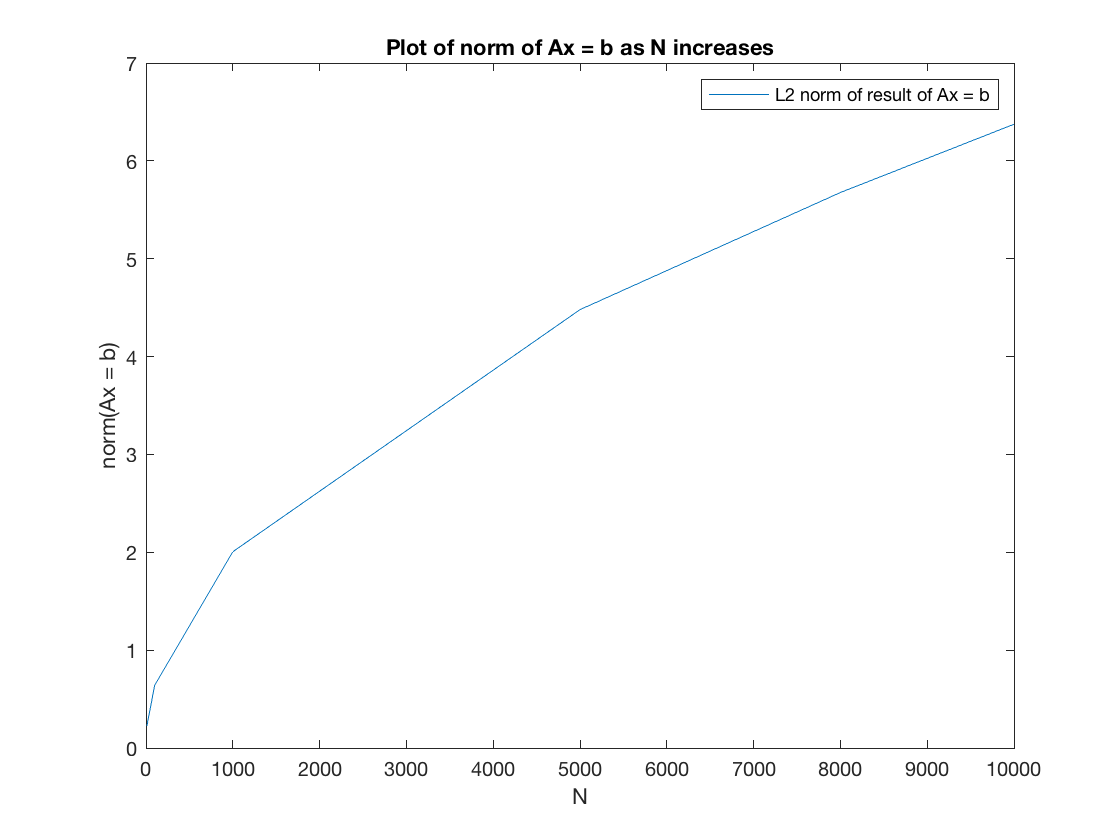
\includegraphics[scale=0.3]{pent_solve_norm.png} \\

\section{}
After using Matlab's backslash to solve Ax = b, it was apparent that the penta solver does compute the same solution as Matlab. Uncomment lines 16 and 17 in main.m to see the comparison side-by-side for each x in Ax = b for size N. Interestingly, Matlab's solver returns results in matrix form, where each column is a duplicate of the results found from using the penta solver.

\section{}
From the figure below, it is apparent that the pentadiagonal solver is faster than the Matlab solver. The Matlab solver timings are not of the same order as the penta solver.  \\

\noindent
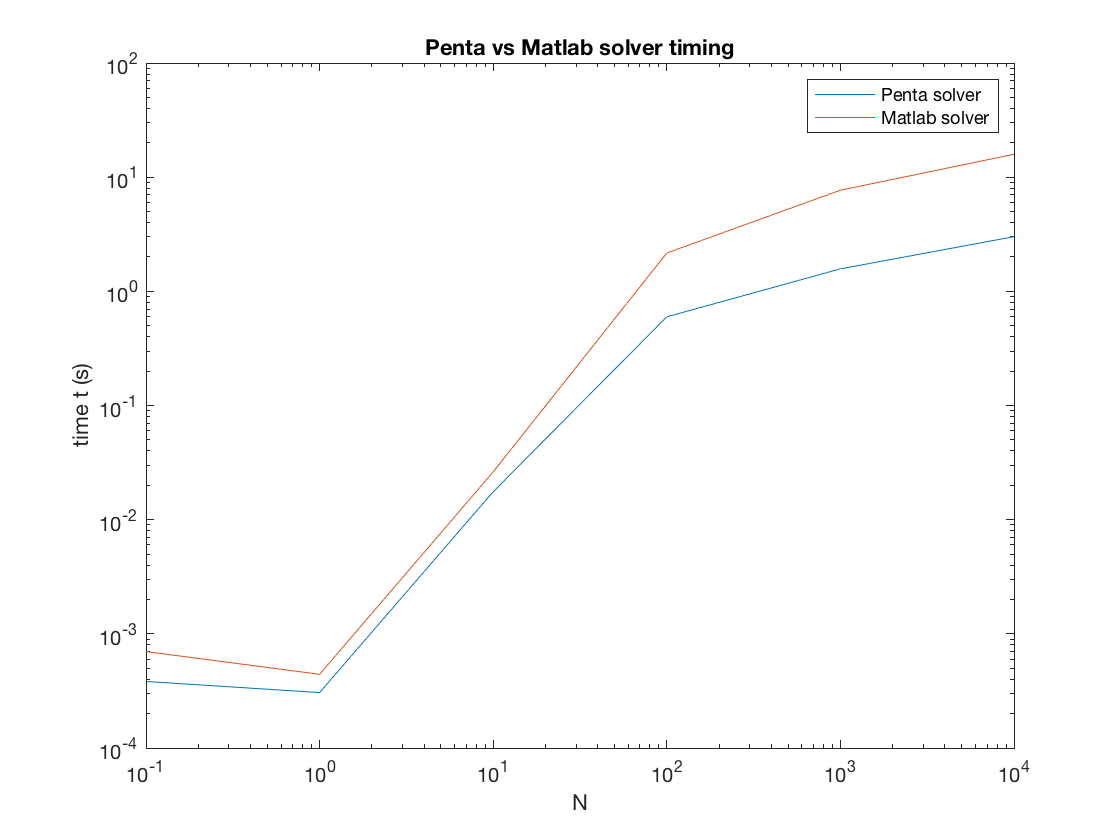
\includegraphics[scale=0.3]{penta_mat_time.png}

\section{}
\section{}
\section{}



\end{document}
